% 西北农林科技大学科技类及IT类课程论文文档类(LaTeX模板)
\documentclass[
  % projtype=paper, % 实习类型,可选report(报告)或paper(论文),默认为report
  % output=epub,     % 输出类型,可选print(打印,不显示超链接颜色)
                   %           或epub(电子稿,显示超链接颜色),默认为epub
  ]{nwafuprojrep}

% 载入需要的宏包
\usepackage{floatrow}% 浮动体增强宏包
\usepackage{subcaption}% 子图排版
\usepackage{amsmath}% 数学宏包
\usepackage{booktabs}% 三线表格
\usepackage{longtable}% 跨页长表格
\usepackage{multirow,makecell}% 表格行合并,单元格处理
\usepackage{ulem}% 下划线
\usepackage[backend=biber,
                style=gb7714-2015,
                maxbibnames=99,% 著录所有作者
                maxcitenames=2,% 引用标注中最多显示2个作者
                mincitenames=1,% 3个及3个以上的作者截断为1个作者
                gbpub=false,
                gbnamefmt=familyahead,
                url=false,
                doi=false,
                isbn=false,
                gbfieldtype=true, % 输出学位论文标识
                ]{biblatex} % 参考文献

% =========命令行窗口及代码排版(自己开发的宏包)=========
% 请确保工作目录中存在boxie.sty、fvextra.sty和lstlinebgrd.sty三个文件
\usepackage{boxie}
% =========插图标注宏包(修改为标注框可以换行)=========
% 请确保工作目录中存在tikz-imglabels.sty文件
\usepackage{tikz-imglabels}
% =========流程图宏包(自己开发)=========
% 请确保工作目录中存在tikz-flowchart.sty文件
\usepackage{tikz-flowchart}

\usepackage{pgf-umlcd}% UML图宏包
\usepackage[ruled,linesnumbered]{algorithm2e}% 算法排版宏包
\usepackage{siunitx}% 标准单位符号宏包
\usepackage{csquotes}% 引号宏包
\usepackage{hyperref}% hyperref 需要最后引入

%%% Local Variables:
%%% mode: latex
%%% TeX-master:"../main.tex"
%%% End:

% 进行必要的设置
% ====================================================================================
% cquotes宏包的中文引号样式
% ====================================================================================
\DeclareQuoteStyle{zhquotestyle}% style name
    {\symbol{"201C}}% opening outer mark
    {\symbol{"201D}}% closing outer mark
    {\symbol{"2018}}% opening inner mark
    {\symbol{"2019}}% closing inner mark

\setquotestyle{zhquotestyle}

% ====================================================================================
% 改变表格字体
% ====================================================================================
\BeforeBeginEnvironment{tabular}{\small}%

% ====================================================================================
% 设置floatrow浮动体属性
% ====================================================================================
\DeclareFloatVCode{beforefig}{\vspace{-4pt}}
\DeclareFloatVCode{beforetab}{\vspace{-6pt}}
\DeclareFloatVCode{afterfloat}{\vspace{4pt}}
\floatsetup{postcode=afterfloat}
\floatsetup[table]{capposition=TOP, captionskip=2pt, objectset=centering, margins=centering, precode=beforetab}
\floatsetup[figure]{captionskip=4pt, objectset=centering, margins=centering, precode=beforefig}

% ====================================================================================
% 代码交叉引用命令\autoref的引用格式
% ====================================================================================
\def\cvcounterautorefname{代码}%
\renewcommand{\thecvcounter}{\arabic{cvcounter}}
\def\cvcounterautorefname~#1\null{代码~#1\null}%

%%% Local Variables:
%%% mode: latex
%%% TeX-master:"../main.tex"
%%% End:

% 专用术语宏命令
% ====================================================================================
% 西北农林科技大学各单位名称
% ====================================================================================
\newcommand{\nwafu}{西北农林科技大学}
\newcommand{\cie}{信息工程学院}

% ============自定义专有名词命令============
\newcommand{\cl}{\texttt{C}语言}
\newcommand{\ccpp}{\texttt{C/C++}}
\newcommand{\win}{\texttt{Windows}}
\newcommand{\ide}{\texttt{IDE}}
\newcommand{\gcc}{\texttt{GCC}}
\newcommand{\gpp}{\texttt{G++}}
\newcommand{\gnu}{\texttt{GNU}}
\newcommand{\cb}{\texttt{Code::Blocks}}
\newcommand{\mgww}{\texttt{MinGW}}
\newcommand{\mgw}{\texttt{MinGW32}}
\newcommand{\mgwww}{\texttt{MinGW-w64}}
\newcommand{\lumos}{\texttt{Linux}、\texttt{Unix}、\texttt{Mac OS}}
\newcommand{\unix}{\texttt{UNIX}}
\newcommand{\lnx}{\texttt{Linux}}
\newcommand{\mk}{\texttt{make}}
\newcommand{\ph}{\texttt{Path}}
\newcommand{\cmdd}{\texttt{cmd}}
\newcommand{\gdb}{\texttt{gdb}调试器}
\newcommand{\vside}{\texttt{Visual Studio}}
\newcommand{\mfile}{\texttt{Makefile}}
\newcommand{\tgt}{\texttt{target}}
\newcommand{\prqt}{\texttt{prerequisites}}
\newcommand{\cbv}{\texttt{17.12}}
\newcommand{\db}{\texttt{DEBUG}}
\newcommand{\dbger}{\texttt{Debugger}}
\newcommand{\cdb}{\texttt{cdb}调试器}
\newcommand{\gdbcmd}{\texttt{(gdb)}}
\newcommand{\bug}{\texttt{BUG}}
\newcommand{\ieee}{\texttt{IEEE754}标准}
\newcommand{\ascii}{\texttt{ASCII}}
\newcommand\vararg{变长形参列表}
\newcommand\varargfun{\vararg{}函数}
\newcommand{\cg}{\texttt{CGraph2D} 图形库}
\newcommand{\git}{分布式版本控制系统\texttt{Git}}
\newcommand{\github}{\texttt{Github}平台}
% ====================================


%%% Local Variables:
%%% mode: latex
%%% TeX-master:"../main.tex"
%%% End:

% 数学符号宏命令
% !TeX root = ./main.tex

% Adapted for use with ustcthesis.
% Original code is at https://github.com/goodfeli/dlbook_notation/blob/master/math_commands.tex

%%%%% NEW MATH DEFINITIONS %%%%%

\newcommand\ceil[1]{\lceil #1 \rceil}
\newcommand\floor[1]{\lfloor #1 \rfloor}


% Vectors
%\newcommand\Vector[1]{\symbf{#1}}

\newcommand\0{{\Vector{0}}}
\newcommand\vzero{{\Vector{0}}}
\newcommand\1{{\Vector{1}}}
\newcommand\vone{{\Vector{1}}}

\newcommand\va{{\Vector{a}}}
\newcommand\vb{{\Vector{b}}}
\newcommand\vc{{\Vector{c}}}
\newcommand\vd{{\Vector{d}}}
\newcommand\ve{{\Vector{e}}}
\newcommand\vf{{\Vector{f}}}
\newcommand\vg{{\Vector{g}}}
\newcommand\vh{{\Vector{h}}}
\newcommand\vi{{\Vector{i}}}
\newcommand\vj{{\Vector{j}}}
\newcommand\vk{{\Vector{k}}}
\newcommand\vl{{\Vector{l}}}
\newcommand\vm{{\Vector{m}}}
\newcommand\vn{{\Vector{n}}}
\newcommand\vo{{\Vector{o}}}
\newcommand\vp{{\Vector{p}}}
\newcommand\vq{{\Vector{q}}}
\newcommand\vr{{\Vector{r}}}
\newcommand\vs{{\Vector{s}}}
\newcommand\vt{{\Vector{t}}}
\newcommand\vu{{\Vector{u}}}
\newcommand\vv{{\Vector{v}}}
\newcommand\vw{{\Vector{w}}}
\newcommand\vx{{\Vector{x}}}
\newcommand\vy{{\Vector{y}}}
\newcommand\vz{{\Vector{z}}}

\newcommand\valpha{{\Vector{\alpha}}}
\newcommand\vbeta{{\Vector{\beta}}}
\newcommand\vgamma{{\Vector{\gamma}}}
\newcommand\vdelta{{\Vector{\delta}}}
\newcommand\vepsilon{{\Vector{\epsilon}}}
\newcommand\vtheta{{\Vector{\theta}}}
\newcommand\viota{{\Vector{\iota}}}
\newcommand\vkappa{{\Vector{\kappa}}}
\newcommand\vlambda{{\Vector{\lambda}}}
\newcommand\vmu{{\Vector{\mu}}}
\newcommand\vnu{{\Vector{\nu}}}
\newcommand\vxi{{\Vector{\xi}}}
\newcommand\vpi{{\Vector{\pi}}}
\newcommand\vrho{{\Vector{\rho}}}
\newcommand\vsigma{{\Vector{\sigma}}}
\newcommand\vtau{{\Vector{\tau}}}
\newcommand\vupsilon{{\Vector{\upsilon}}}
\newcommand\vphi{{\Vector{\phi}}}
\newcommand\vchi{{\Vector{\chi}}}
\newcommand\vpsi{{\Vector{\psi}}}
\newcommand\vomega{{\Vector{\omega}}}


% Matrix
\newcommand\MATRIX[1]{\symbf{#1}}

\newcommand\mA{{\MATRIX{A}}}
\newcommand\mB{{\MATRIX{B}}}
\newcommand\mC{{\MATRIX{C}}}
\newcommand\mD{{\MATRIX{D}}}
\newcommand\mE{{\MATRIX{E}}}
\newcommand\mF{{\MATRIX{F}}}
\newcommand\mG{{\MATRIX{G}}}
\newcommand\mH{{\MATRIX{H}}}
\newcommand\mI{{\MATRIX{I}}}
\newcommand\mJ{{\MATRIX{J}}}
\newcommand\mK{{\MATRIX{K}}}
\newcommand\mL{{\MATRIX{L}}}
\newcommand\mM{{\MATRIX{M}}}
\newcommand\mN{{\MATRIX{N}}}
\newcommand\mO{{\MATRIX{O}}}
\newcommand\mP{{\MATRIX{P}}}
\newcommand\mQ{{\MATRIX{Q}}}
\newcommand\mR{{\MATRIX{R}}}
\newcommand\mS{{\MATRIX{S}}}
\newcommand\mT{{\MATRIX{T}}}
\newcommand\mU{{\MATRIX{U}}}
\newcommand\mV{{\MATRIX{V}}}
\newcommand\mW{{\MATRIX{W}}}
\newcommand\mX{{\MATRIX{X}}}
\newcommand\mY{{\MATRIX{Y}}}
\newcommand\mZ{{\MATRIX{Z}}}

\newcommand\mGamma{{\MATRIX{\Gamma}}}
\newcommand\mDelta{{\MATRIX{\Delta}}}
\newcommand\mTheta{{\MATRIX{\Theta}}}
\newcommand\mLambda{{\MATRIX{\Lambda}}}
\newcommand\mXi{{\MATRIX{\Xi}}}
\newcommand\mPi{{\MATRIX{\Pi}}}
\newcommand\mSigma{{\MATRIX{\Sigma}}}
\newcommand\mUpsilon{{\MATRIX{\Upsilon}}}
\newcommand\mPhi{{\MATRIX{\Phi}}}
\newcommand\mPsi{{\MATRIX{\Psi}}}
\newcommand\mOmega{{\MATRIX{\Omega}}}


% Tensor
\newcommand\tens[1]{\symbfsf{#1}}
\newcommand\tA{{\tens{A}}}
\newcommand\tB{{\tens{B}}}
\newcommand\tC{{\tens{C}}}
\newcommand\tD{{\tens{D}}}
\newcommand\tE{{\tens{E}}}
\newcommand\tF{{\tens{F}}}
\newcommand\tG{{\tens{G}}}
\newcommand\tH{{\tens{H}}}
\newcommand\tI{{\tens{I}}}
\newcommand\tJ{{\tens{J}}}
\newcommand\tK{{\tens{K}}}
\newcommand\tL{{\tens{L}}}
\newcommand\tM{{\tens{M}}}
\newcommand\tN{{\tens{N}}}
\newcommand\tO{{\tens{O}}}
\newcommand\tP{{\tens{P}}}
\newcommand\tQ{{\tens{Q}}}
\newcommand\tR{{\tens{R}}}
\newcommand\tS{{\tens{S}}}
\newcommand\tT{{\tens{T}}}
\newcommand\tU{{\tens{U}}}
\newcommand\tV{{\tens{V}}}
\newcommand\tW{{\tens{W}}}
\newcommand\tX{{\tens{X}}}
\newcommand\tY{{\tens{Y}}}
\newcommand\tZ{{\tens{Z}}}


% Graph
\newcommand\gA{{\mathcal{A}}}
\newcommand\gB{{\mathcal{B}}}
\newcommand\gC{{\mathcal{C}}}
\newcommand\gD{{\mathcal{D}}}
\newcommand\gE{{\mathcal{E}}}
\newcommand\gF{{\mathcal{F}}}
\newcommand\gG{{\mathcal{G}}}
\newcommand\gH{{\mathcal{H}}}
\newcommand\gI{{\mathcal{I}}}
\newcommand\gJ{{\mathcal{J}}}
\newcommand\gK{{\mathcal{K}}}
\newcommand\gL{{\mathcal{L}}}
\newcommand\gM{{\mathcal{M}}}
\newcommand\gN{{\mathcal{N}}}
\newcommand\gO{{\mathcal{O}}}
\newcommand\gP{{\mathcal{P}}}
\newcommand\gQ{{\mathcal{Q}}}
\newcommand\gR{{\mathcal{R}}}
\newcommand\gS{{\mathcal{S}}}
\newcommand\gT{{\mathcal{T}}}
\newcommand\gU{{\mathcal{U}}}
\newcommand\gV{{\mathcal{V}}}
\newcommand\gW{{\mathcal{W}}}
\newcommand\gX{{\mathcal{X}}}
\newcommand\gY{{\mathcal{Y}}}
\newcommand\gZ{{\mathcal{Z}}}


% Sets
\newcommand\sA{{\mathbb{A}}}
\newcommand\sB{{\mathbb{B}}}
\newcommand\sC{{\mathbb{C}}}
\newcommand\sD{{\mathbb{D}}}
% Don't use a set called E, because this would be the same as our symbol
% for expectation.
\newcommand\sF{{\mathbb{F}}}
\newcommand\sG{{\mathbb{G}}}
\newcommand\sH{{\mathbb{H}}}
\newcommand\sI{{\mathbb{I}}}
\newcommand\sJ{{\mathbb{J}}}
\newcommand\sK{{\mathbb{K}}}
\newcommand\sL{{\mathbb{L}}}
\newcommand\sM{{\mathbb{M}}}
\newcommand\sN{{\mathbb{N}}}
\newcommand\sO{{\mathbb{O}}}
\newcommand\sP{{\mathbb{P}}}
\newcommand\sQ{{\mathbb{Q}}}
\newcommand\sR{{\mathbb{R}}}
\newcommand\sS{{\mathbb{S}}}
\newcommand\sT{{\mathbb{T}}}
\newcommand\sU{{\mathbb{U}}}
\newcommand\sV{{\mathbb{V}}}
\newcommand\sW{{\mathbb{W}}}
\newcommand\sX{{\mathbb{X}}}
\newcommand\sY{{\mathbb{Y}}}
\newcommand\sZ{{\mathbb{Z}}}


% Random variables
\newcommand\RandomVariable[1]{\symit{#1}}

\newcommand\rA{{\RandomVariable{A}}}
\newcommand\rB{{\RandomVariable{B}}}
\newcommand\rC{{\RandomVariable{C}}}
\newcommand\rD{{\RandomVariable{D}}}
\newcommand\rE{{\RandomVariable{E}}}
\newcommand\rF{{\RandomVariable{F}}}
\newcommand\rG{{\RandomVariable{G}}}
\newcommand\rH{{\RandomVariable{H}}}
\newcommand\rI{{\RandomVariable{I}}}
\newcommand\rJ{{\RandomVariable{J}}}
\newcommand\rK{{\RandomVariable{K}}}
\newcommand\rL{{\RandomVariable{L}}}
\newcommand\rM{{\RandomVariable{M}}}
\newcommand\rN{{\RandomVariable{N}}}
\newcommand\rO{{\RandomVariable{O}}}
\newcommand\rP{{\RandomVariable{P}}}
\newcommand\rQ{{\RandomVariable{Q}}}
\newcommand\rR{{\RandomVariable{R}}}
\newcommand\rS{{\RandomVariable{S}}}
\newcommand\rT{{\RandomVariable{T}}}
\newcommand\rU{{\RandomVariable{U}}}
\newcommand\rV{{\RandomVariable{V}}}
\newcommand\rW{{\RandomVariable{W}}}
\newcommand\rX{{\RandomVariable{X}}}
\newcommand\rY{{\RandomVariable{Y}}}
\newcommand\rZ{{\RandomVariable{Z}}}

% Random vectors
\newcommand\RandomVector[1]{\symbf{#1}}

\newcommand\rvA{{\RandomVector{A}}}
\newcommand\rvB{{\RandomVector{B}}}
\newcommand\rvC{{\RandomVector{C}}}
\newcommand\rvD{{\RandomVector{D}}}
\newcommand\rvE{{\RandomVector{E}}}
\newcommand\rvF{{\RandomVector{F}}}
\newcommand\rvG{{\RandomVector{G}}}
\newcommand\rvH{{\RandomVector{H}}}
\newcommand\rvI{{\RandomVector{I}}}
\newcommand\rvJ{{\RandomVector{J}}}
\newcommand\rvK{{\RandomVector{K}}}
\newcommand\rvL{{\RandomVector{L}}}
\newcommand\rvM{{\RandomVector{M}}}
\newcommand\rvN{{\RandomVector{N}}}
\newcommand\rvO{{\RandomVector{O}}}
\newcommand\rvP{{\RandomVector{P}}}
\newcommand\rvQ{{\RandomVector{Q}}}
\newcommand\rvR{{\RandomVector{R}}}
\newcommand\rvS{{\RandomVector{S}}}
\newcommand\rvT{{\RandomVector{T}}}
\newcommand\rvU{{\RandomVector{U}}}
\newcommand\rvV{{\RandomVector{V}}}
\newcommand\rvW{{\RandomVector{W}}}
\newcommand\rvX{{\RandomVector{X}}}
\newcommand\rvY{{\RandomVector{Y}}}
\newcommand\rvZ{{\RandomVector{Z}}}

\newcommand\laplace{\mathrm{Laplace}} % Laplace distribution

\newcommand\E{\mathbb{E}}
\newcommand\Ls{\mathcal{L}}
\newcommand\R{\mathbb{R}}
\newcommand\emp{\tilde{p}}
\newcommand\lr{\alpha}
\newcommand\reg{\lambda}
\newcommand\rect{\mathrm{rectifier}}
\newcommand\softmax{\mathrm{softmax}}
\newcommand\sigmoid{\sigma}
\newcommand\softplus{\zeta}
\newcommand\KL{D_{\mathrm{KL}}}
\newcommand\Var{\mathrm{Var}}
\newcommand\standarderror{\mathrm{SE}}
\newcommand\Cov{\mathrm{Cov}}
% Wolfram Mathworld says $L^2$ is for function spaces and $\ell^2$ is for vectors
% But then they seem to use $L^2$ for vectors throughout the site, and so does
% wikipedia.
\newcommand\normlzero{L^0}
\newcommand\normlone{L^1}
\newcommand\normltwo{L^2}
\newcommand\normlp{L^p}
\newcommand\normmax{L^\infty}

\DeclareMathOperator*{\argmax}{arg\,max}
\DeclareMathOperator*{\argmin}{arg\,min}

\DeclareMathOperator{\sign}{sign}
\DeclareMathOperator{\Tr}{Tr}
\let\ab\allowbreak


% 设置封面基本信息,\linebreak 前面不要有空格,
% 中文之间的空格无法消除
% 另,在\nwafuset中不可以出现空行
\nwafuset{
  college = {信息工程学院},            % 学院名称
  projname = {\LaTeX{}科技排版},       % 实践课程名称
  title = {\LaTeX{}科技排版实习报告},  % 实习报告题目
  stuno = {2013051289},              % 学号
  author = {\LaTeX{}er},             % 姓名
  major = {计算机科学与技术},          % 专业
  classid = {152},                   % 班级(只填写数字,不要有其它内容)
  adviser = {Registor},                   % 指导教师姓名
  startdate = {2020年8月10日},        % 实践起始日期
  enddate = {8月23日},        % 实践结束日期
}

%biblatex宏包的参考文献数据源加载方式
\addbibresource[location=local]{bib/example.bib}
\begin{document} %在document环境中撰写文档

%%%%%%%%%%%%%%%%%%%%%%%%%%%%%%%%%%%%%%%%
% 封面及目录,无需改动此处代码
% 面页,需要在导言区用\nwafuset命令填写基本信息
\makecover
% 目录
\tableofcontents
\cleardoublepage
% 设置正文页眉页脚格式,并重新设置页码为1
\pagestyle{main}% 无页眉,页码在页脚居中
%%%%%%%%%%%%%%%%%%%%%%%%%%%%%%%%%%%%%%%%


% 排版摘要
% 摘要内容
\begin{abstract}
  针对课程综合实习实习报告(或论文)排版中的格式问题,基于\emph{内容与格式分离}的\LaTeX{}排版技术,通分析西北农林科技大学信息工程学院给出的课程综合实习实习报告(或论文)排版规范和样例文件,采用文档类的方式,结合作者前期开发的boxie、tikz-flowchart、tikz-imglabels等宏包,设计并开发了\enquote{nwafuprojrep.cls}西北农林科技大学信息工程学院课程综合实习实习报告(或论文)\LaTeX{}模板。该模板能够根据操作系统自动选择需要的字体,提供了基本的格式限定及代码、流程图绘制、图像标注等实用功能。测试结果表明,该模板在Ubuntu、Winodws、Mac下均可以按规范实现实习报告(或论文)的正确排版。
\end{abstract}
% 关键词内容(不同关键字,请用英文","分割)
\keywords{\LaTeX{}模板, 文档类, 宏包, 实习报告}
\makeabstract

% 排版正文内容
\section{综合训练目的与要求}
该综合训练的目的是培养应用《\LaTeX{}科技排版》设计方法及思想解决实际问
题的能力,掌握使用\LaTeX{}科技排版技术,熟悉开发工具的使用。同时提升级
调查研究、查阅文献及编写技术文档的能力。
\section{综合训练任务}
根据指定的题目要求,完成功能设计;选择合适的平台和工具实现代码编写和调
试;设计合理的测试方案,对设计的代码进行完整测试。
\section{总体设计}
西北农林科技大学信息工程学院实习报告撰写规范和样例进行\LaTeX{}
nwafuprojrep模板的开发。

在设计中,以\emph{内容与格式分离}为原则,主要对标题格式、图表浮动体、交
叉引用、参考文献等格式进行了限定,以减轻排版中的格式设置与调整工作量。

\section{详细设计说明}
\subsection{插图浮动体}
在\enquote{nwafuprojrep.cls}模板中,除了可以使用普通的figure浮动体环境
结合graphicx宏包实现插图排版外,还可以使用floatrow增强浮动体宏包进行浮
动体排版(适合多图并排、子图排版等)。有关该宏包的使用细节,请在命令行使
用\enquote{texdoc floatrow}命令查看其使用说明书。例如,可以
用\autoref{texcode01}排版\autoref{sharefig:a}。

% 该center环境中的代码为排版示例代码,实际排版中不需要该代码
\begin{center}
\begin{langCVOne}[tex][texcode01][\LaTeX{}]{排版单一插图浮动体}
  \begin{figure}[!htp]
    \begin{floatrow}
      \ffigbox[\FBwidth]{
        \includegraphics[width=0.4\textwidth]{example-image-a}
      }{\caption{一个插图}\label{sharefig:a}}
    \end{floatrow}
  \end{figure}
\end{langCVOne}
\end{center}

\begin{figure}[!htp]
  \begin{floatrow}
    \ffigbox[\FBwidth]{
      \includegraphics[width=0.4\textwidth]{example-image-a}
    }{\caption{一个插图}\label{sharefig:a}}
  \end{floatrow}
\end{figure}

当然,也可以用\autoref{texcode02}排版带有子图的\autoref{trifig}。  

% 该center环境中的代码为排版示例代码,实际排版中不需要该代码
\begin{center}
\begin{langCVOne}[tex][texcode02][\LaTeX{}]{排版单一插图浮动体}
\begin{figure}[!htp]
  \ffigbox[\textwidth]%
  {%
    \begin{subfloatrow}[2]%\useFCwidth
      \ffigbox[\FBwidth]{
        \includegraphics[width=0.3\textwidth]{example-image-a}
      }{\caption{子题注1}\label{trifig:a}}
      \ffigbox[\FBwidth]{
        \includegraphics[width=0.3\textwidth]{example-image-b}
      }{\caption{子题注2}\label{trifig:b}}
    \end{subfloatrow}    
    \begin{subfloatrow}[2]%\useFCwidth      
      \ffigbox[\FBwidth]{
        \includegraphics[width=0.3\textwidth]{example-image-c}
      }{\caption{子题注3}\label{trifig:c}}
      \ffigbox[\FBwidth]{
        \includegraphics[width=0.3\textwidth]{example-image}
      }{\caption{子题注4}\label{trifig:d}}
    \end{subfloatrow}
  }{\caption{四个子图}\label{trifig}}
\end{figure}
\end{langCVOne}
\end{center}

\begin{figure}[!htp]
  \ffigbox[\textwidth]%
  {%
    \begin{subfloatrow}[2]%\useFCwidth
      \ffigbox[\FBwidth]{
        \includegraphics[width=0.25\textwidth]{example-image-a}
      }{\caption{子题注1}\label{trifig:a}}
      \ffigbox[\FBwidth]{
        \includegraphics[width=0.25\textwidth]{example-image-b}
        
      }{\caption{子题注2}\label{trifig:b}}
    \end{subfloatrow}    
    \begin{subfloatrow}[2]%\useFCwidth      
      \ffigbox[\FBwidth]{
        \includegraphics[width=0.25\textwidth]{example-image-c}
      }{\caption{子题注3}\label{trifig:c}}
      \ffigbox[\FBwidth]{
        \includegraphics[width=0.25\textwidth]{example-image}
      }{\caption{子题注4}\label{trifig:d}}
    \end{subfloatrow}
  }{\caption{四个子图}\label{trifig}}
\end{figure}

在模板中,已为插图设置
了{{./figs/}、{./figure/}、{./figures/}、{./image/}、{./images/}、
  {./graphics/}、{./graphic/}、{./pictures/}、{./picture/}}相对路径,可
以在当前工作路径中任意一个这样命名的文件夹,以存放需要的插图文件。

\subsection{表格浮动体}
如果需要插入一个简单的表格,可以仅使用{table}和{tabular}环境实现,如%
\autoref{tab:city}。

\emph{注意:}科技文档中的表格需要采用\emph{三线表}。

\begin{table}[!htb]
  \caption[城市人口]{城市人口数量排名 (source: Wikipedia)\label{tab:city}}
  \begin{tabular}{lr}
    \toprule
    城市 & 人口 \\
    \midrule
    Mexico City & 20,116,842\\
    Shanghai & 19,210,000\\
    Peking & 15,796,450\\
    Istanbul & 14,160,467\\
    \bottomrule
  \end{tabular}
\end{table}

如果多个表格布局较为复杂,可以使用floatrow宏包实现排版。如%
用\autoref{texcodetab}可编制\autoref{tab:testsample}和%
\autoref{tab:city2}所示的横向并排表格。%

% 该center环境中的代码为排版示例代码,实际排版中不需要该代码
\begin{center}
  \begin{langCVOne}[tex][texcodetab][\LaTeX{}]{表格排版}
    % 横向排版两个表格
    \begin{table}[!htp]
      \begin{floatrow}
        \ttabbox[\FBwidth]
        {
          \begin{tabular}{ccl}
            \toprule
            序号 & 测试用例 & \multicolumn{1}{c}{测试目的}\\
            \midrule
            1 & a & 小写字母到大写字母转换\\
            2 & A & 大写字母到小写字母转换\\
            3 & @ & 非字母字符测试\\
            4 & 2 & 非字母其它字符\\
            \bottomrule
          \end{tabular}      
        }{\caption{字母大小写转换测试用例表}\label{tab:testsample}}
        \ttabbox[\FBwidth]
        {
          \begin{tabular}{lr}
            \toprule
            城市 & 人口 \\
            \midrule
            Mexico City & 20,116,842\\
            Shanghai & 19,210,000\\
            Peking & 15,796,450\\
            Istanbul & 14,160,467\\
            \bottomrule
          \end{tabular}      
        }{\caption{城市人口数量排名}\label{tab:city2}}
      \end{floatrow}
    \end{table}
  \end{langCVOne}
\end{center}

% 横向排版两个表格
\begin{table}[!htp]
  \begin{floatrow}
    \ttabbox[\FBwidth]
    {
      \begin{tabular}{ccl}
        \toprule
        序号 & 测试用例 & \multicolumn{1}{c}{测试目的}\\
        \midrule
        1 & a & 小写字母到大写字母转换\\
        2 & A & 大写字母到小写字母转换\\
        3 & @ & 非字母字符测试\\
        4 & 2 & 非字母其它字符\\
        \bottomrule
      \end{tabular}      
    }{\caption{字母大小写转换测试用例表}\label{tab:testsample}}
    \ttabbox[\FBwidth]
    {
      \begin{tabular}{lr}
        \toprule
        城市 & 人口 \\
        \midrule
        Mexico City & 20,116,842\\
        Shanghai & 19,210,000\\
        Peking & 15,796,450\\
        Istanbul & 14,160,467\\
        \bottomrule
      \end{tabular}      
    }{\caption{城市人口数量排名}\label{tab:city2}}
  \end{floatrow}
\end{table}

% \begin{table}[!htp]
%   \ttabbox[\FBwidth]{
%     \begin{tabular}{ccl}
%       \toprule
%       序号 & 测试用例 & \multicolumn{1}{c}{测试目的}\\
%       \midrule
%       1 & a & 小写字母到大写字母转换\\
%       2 & A & 大写字母到小写字母转换\\
%       3 & @ & 非字母字符测试\\
%       4 & 2 & 非字母其它字符\\
%       \bottomrule      
%     \end{tabular}
%   }{\caption{字母大小写转换测试用例表}\label{tab:testsample}}
% \end{table}

如果表格内容很多,导致无法放在一页内的话,需要用{longtable} 或{longtabu} 进行分页。
\autoref{tab:performance}是一个长表格的例子。

% 定义表中用到的的宏,以简化表格代码并为后续修改提供统一接口
\def\tabcaption{实验数据,这个题注十分的长,注意这在索引中的处理方式,还有 \cs{caption} 后面的双反斜杠}
\def\tabheadrow{
  \multirow{2}{*}{测试程序} & \multicolumn{1}{c}{正常运行} &
   \multicolumn{1}{c}{同步} & \multicolumn{1}{c}{检查点} &
   \multicolumn{1}{c}{卷回恢复} & \multicolumn{1}{c}{进程迁移} &
   \multicolumn{1}{c}{检查点} \\
   & \multicolumn{1}{c}{时间(s)} & \multicolumn{1}{c}{时间(s)} &
   \multicolumn{1}{c}{时间(s)} & \multicolumn{1}{c}{时间(s)} &
   \multicolumn{1}{c}{时间(s)} & \multicolumn{1}{c}{文件(KB)} \\
 }

% 定义跨页表续表表题
\def\ctntabcap{
   \multicolumn{7}{c}{\small\heiti{}续表~\thetable\hskip1em 实验测试数据}  
 }
 % 定义跨页表命令集合
\def\ctntabcmd{
   \\\ctntabcap\\
   \toprule
   \tabheadrow
   \midrule
   \endhead
   \midrule
   \multicolumn{7}{r}{续下页}\\
   \endfoot
   \endlastfoot  
 } 
 
 
\begin{longtable}[c]{c*{6}{r}}
        \caption[实验数据]{实验测试数据}\label{tab:performance}\\
        \toprule
        \tabheadrow
        \midrule
        \endfirsthead
        \ctntabcmd
        CG.A.2 & 23.05 & 0.002 & 0.116 & 0.035 & 0.589 & 32491 \\
        CG.A.4 & 15.06 & 0.003 & 0.067 & 0.021 & 0.351 & 18211 \\
        CG.A.8 & 13.38 & 0.004 & 0.072 & 0.023 & 0.210 & 9890 \\
        CG.B.2 & 867.45 & 0.002 & 0.864 & 0.232 & 3.256 & 228562 \\
        CG.B.4 & 501.61 & 0.003 & 0.438 & 0.136 & 2.075 & 123862 \\
        CG.B.8 & 384.65 & 0.004 & 0.457 & 0.108 & 1.235 & 63777 \\
        MG.A.2 & 112.27 & 0.002 & 0.846 & 0.237 & 3.930 & 236473 \\
        MG.A.4 & 59.84 & 0.003 & 0.442 & 0.128 & 2.070 & 123875 \\
        MG.A.8 & 31.38 & 0.003 & 0.476 & 0.114 & 1.041 & 60627 \\
        MG.B.2 & 526.28 & 0.002 & 0.821 & 0.238 & 4.176 & 236635 \\
        MG.B.4 & 280.11 & 0.003 & 0.432 & 0.130 & 1.706 & 123793 \\
        MG.B.8 & 148.29 & 0.003 & 0.442 & 0.116 & 0.893 & 60600 \\
        LU.A.2 & 2116.54 & 0.002 & 0.110 & 0.030 & 0.532 & 28754 \\
        LU.A.4 & 1102.50 & 0.002 & 0.069 & 0.017 & 0.255 & 14915 \\
        LU.A.8 & 574.47 & 0.003 & 0.067 & 0.016 & 0.192 & 8655 \\
        LU.B.2 & 9712.87 & 0.002 & 0.357 & 0.104 & 1.734 & 101975 \\
        LU.B.4 & 4757.80 & 0.003 & 0.190 & 0.056 & 0.808 & 53522 \\
        LU.B.8 & 2444.05 & 0.004 & 0.222 & 0.057 & 0.548 & 30134 \\
        CG.B.2 & 867.45 & 0.002 & 0.864 & 0.232 & 3.256 & 228562 \\
        CG.B.4 & 501.61 & 0.003 & 0.438 & 0.136 & 2.075 & 123862 \\
        CG.B.8 & 384.65 & 0.004 & 0.457 & 0.108 & 1.235 & 63777 \\
        MG.A.2 & 112.27 & 0.002 & 0.846 & 0.237 & 3.930 & 236473 \\
        MG.A.4 & 59.84 & 0.003 & 0.442 & 0.128 & 2.070 & 123875 \\
        MG.A.8 & 31.38 & 0.003 & 0.476 & 0.114 & 1.041 & 60627 \\
        MG.B.2 & 526.28 & 0.002 & 0.821 & 0.238 & 4.176 & 236635 \\
        MG.B.4 & 280.11 & 0.003 & 0.432 & 0.130 & 1.706 & 123793 \\
        MG.B.8 & 148.29 & 0.003 & 0.442 & 0.116 & 0.893 & 60600 \\
        LU.A.2 & 2116.54 & 0.002 & 0.110 & 0.030 & 0.532 & 28754 \\
        LU.A.4 & 1102.50 & 0.002 & 0.069 & 0.017 & 0.255 & 14915 \\
        LU.A.8 & 574.47 & 0.003 & 0.067 & 0.016 & 0.192 & 8655 \\
        LU.B.2 & 9712.87 & 0.002 & 0.357 & 0.104 & 1.734 & 101975 \\
        LU.B.4 & 4757.80 & 0.003 & 0.190 & 0.056 & 0.808 & 53522 \\
        LU.B.8 & 2444.05 & 0.004 & 0.222 & 0.057 & 0.548 & 30134 \\
        EP.A.2 & 123.81 & 0.002 & 0.010 & 0.003 & 0.074 & 1834 \\
        EP.A.4 & 61.92 & 0.003 & 0.011 & 0.004 & 0.073 & 1743 \\
        EP.A.8 & 31.06 & 0.004 & 0.017 & 0.005 & 0.073 & 1661 \\
        EP.B.2 & 495.49 & 0.001 & 0.009 & 0.003 & 0.196 & 2011 \\
        EP.B.4 & 247.69 & 0.002 & 0.012 & 0.004 & 0.122 & 1663 \\
        EP.B.8 & 126.74 & 0.003 & 0.017 & 0.005 & 0.083 & 1656 \\
        \bottomrule
   \end{longtable}

\subsection{插图标注}
在\enquote{nwafuprojrep.cls}模板中,可能通过引入了改自tikz-imagelabels宏包
的tikz-imglabels宏包,利用TikZ为插图进行标注。该宏包的使用细节与
tikz-imagelabels完全一致,请在命令行使用\enquote{texdoc tikz-imagelabels}命令
查看其使用说明书。\autoref{texcode03}用于实现\autoref{fig:annot}所示的插图标注。

% 该center环境中的代码为排版示例代码,实际排版中不需要该代码
\begin{center}
\begin{langCVOne}[tex][texcode03][\LaTeX{}]{插图标注代码}
\begin{figure}[!htp]
  \centering
    \begin{annotationimage}{width=0.8\textwidth}{figs/01reviewicons01}
      % 绘制外观设置按钮分组示意下划线
      \draw[thick,blue] (0.86,0.26) -- (1.0,0.26);
      % 添加各图标标注
      \foreach \ann/\xpos in
      {
        {附\\注\\工\\具}/0.02, {高\\亮\\工\\具}/0.07,
        {下\\划\\线\\工\\具}/0.126, {删\\除\\线\\工\\具}/0.18,
        {删\\除\\线\\并\\插\\入\\附\\注\\工\\具}/0.229, {插\\入\\文\\本\\工\\具}/0.283,
        {文\\本\\工\\具}/0.346, {文\\本\\框\\工\\具}/0.40,
        {铅\\笔\\绘\\图\\工\\具}/0.45, {铅\\笔\\擦\\工\\具}/0.51,
        {图\\章\\工\\具}/0.56, {附\\加\\文\\件\\工\\具}/0.63,
        {绘\\图\\工\\具}/0.7, {保\\持\\选\\择\\工\\具}/0.79,
        {注\\释\\外\\观\\设\\置}/0.93
      }
      {
        \draw[annotation below = {{\ann} at \xpos}] to (\xpos,0.48);
      }
    \end{annotationimage}
    \caption{插图标注}\label{fig:annot}
  \end{figure}
\end{langCVOne}
\end{center}

% 图像标注
\begin{figure}[!htp]
  \centering
  \begin{annotationimage}{width=0.8\textwidth}{figs/01reviewicons01}
    % 绘制外观设置按钮分组示意下划线
    \draw[thick,blue] (0.86,0.26) -- (1.0,0.26);
    % 添加各图标标注
    \foreach \ann/\xpos in
    {
      {附\\注\\工\\具}/0.02, {高\\亮\\工\\具}/0.07,
      {下\\划\\线\\工\\具}/0.126, {删\\除\\线\\工\\具}/0.18,
      {删\\除\\线\\并\\插\\入\\附\\注\\工\\具}/0.229, {插\\入\\文\\本\\工\\具}/0.283,
      {文\\本\\工\\具}/0.346, {文\\本\\框\\工\\具}/0.40,
      {铅\\笔\\绘\\图\\工\\具}/0.45, {铅\\笔\\擦\\工\\具}/0.51,
      {图\\章\\工\\具}/0.56, {附\\加\\文\\件\\工\\具}/0.63,
      {绘\\图\\工\\具}/0.7, {保\\持\\选\\择\\工\\具}/0.79,
      {注\\释\\外\\观\\设\\置}/0.93
    }
    {
      \draw[annotation below = {{\ann} at \xpos}] to (\xpos,0.48);
    }
  \end{annotationimage}
  \caption{插图标注}\label{fig:annot}
\end{figure}

\subsection{流程图}
在\enquote{nwafuprojrep.cls}模板中,可能引入了自己开发
的tikz-flowchart宏包进行流程图的绘制。请
在\github{}查看%
\href{https://github.com/registor/tikz-flowchart}{tikz-flowchart宏包}的
使用说明书。

在绘制流程图时,可以先用纸和笔绘制草稿,然后根据草稿布置各个结点,再
连接流程线。这样,可以做到心中有数,绘制较为方便。

\autoref{subfig:draft}是一个流程图草稿。根据该草稿,基于tikz-flowchart宏包,
用\autoref{texcode04}可绘制\autoref{subfig:tikz}所示的流程图。

% 该center环境中的代码为排版示例代码,实际排版中不需要该代码
\begin{center}
  \begin{langCVOne}[tex][texcode04][\LaTeX{}]{绘制流程图}
    % 流程图绘制属性设置
    \flowchartset{
      proc fill color = orange!10, % 顺序处理框填充颜色(默认取白色)
      test fill color = green!30, % 判断框填充颜色(默认取白色)
      io fill color = blue!30, % 输入/输出框填充颜色(默认取白色)
      term fill color = red!30, % 开始/结束框填充颜色(默认取白色)
    }
    % 绘制流程图
    \begin{tikzpicture}[scale=0.53,transform shape,]
      % 布置结点单元
      \node [term] (st) {开始};
      \node [proc, text width = 5em, join] (p1) {int divisor};       
      \node [test, join] (t1) {n <= 1};
      \node [proc, text width = 5em] (p2) {divisor = 2};
      \node [test, text width = 10em, join] (t2) {divisor * divisor <= n};
      \node [test, text width = 8em] (t3) {n \% divisor == 0};
      \node [proc, text width = 5em] (p3) {divisor++};
      \node [term, below = 1.6 of p3] (end) {结束};
      \node [proc, text width = 4em, left = 4.8 of t2] (p4) {return 0};
      \node [proc, text width = 4em, right = 3.5 of p3] (p5) {return 0};
      \node [proc, text width = 4em, right = 5.8 of t3] (p6) {return 1};

      % 布置用于连接的坐标结点,同时为其布置调试标记点。
      \node [coord] (c1) at ($(p2.south)!0.5!(t2.north)$)  {}; \cmark{1}
      \node [coord, below = 0.25 of p3] (c2)  {}; \cmark{2}
      \node [coord, above = 0.5 of end] (c3) {};  \cmark{3}
      \node [coord, left = 0.5 of t2] (ct) {};  \cmark{t}
      \node [coord] (c4) at (c3 -| p5)  {}; \cmark{4}
      \node [coord] (c5) at (c2 -| ct)  {}; \cmark{5}
        
      % 判断框连线,每次绘制时,先绘制一个带有一个固定
      % 位置标注的路径(path),然后再绘制箭头本身(arrow)。
      \path (t1.south) -- node [near start, right] {$N$} (p2.north);
      \draw [norm] (t1.south) -- (p2.north);
      \path (t1.west) -| node [near start, above] {$Y$} (p4.north);
      \draw [norm] (t1.west) -| (p4.north);
      
      \path (t2.south) -- node [near start, right] {$Y$} (t3.north);
      \draw [norm] (t2.south) -- (t3.north);
      \path (t2.east) -| node [near start, above] {$N$} (p6.north);
      \draw [norm] (t2.east) -| (p6.north);
      
      \path (t3.south) -- node [near start, right] {$N$} (p3.north);
      \draw [norm] (t3.south) -- (p3.north);
      \path (t3.east) -| node [near start, above] {$Y$} (p5.north);
      \draw [norm] (t3.east) -| (p5.north);

      % 其它连线
      \draw [norm](p3.south) |- (c5) |- (c1);
      \draw [norm](p4.south) |- (c3);
      \draw [norm](p4.south) |- (c3) -- (end);
      \draw [norm](p5.south) -- (c4);
      \draw [norm](p6.south) |- (c3);
      \draw [norm](p6.south) |- (c3) -- (end);
    \end{tikzpicture}
  \end{langCVOne}
\end{center}

% 流程图绘制属性设置
\flowchartset{
  proc fill color = orange!10, % 顺序处理框填充颜色(默认取白色)
  test fill color = green!30, % 判断框填充颜色(默认取白色)
  io fill color = blue!30, % 输入/输出框填充颜色(默认取白色)
  term fill color = red!30, % 开始/结束框填充颜色(默认取白色)
}

\begin{figure}[!htp]
  \ffigbox[\textwidth]%
  {%
    \begin{subfloatrow}[2]%\useFCwidth
      \ffigbox[\FBwidth]{
        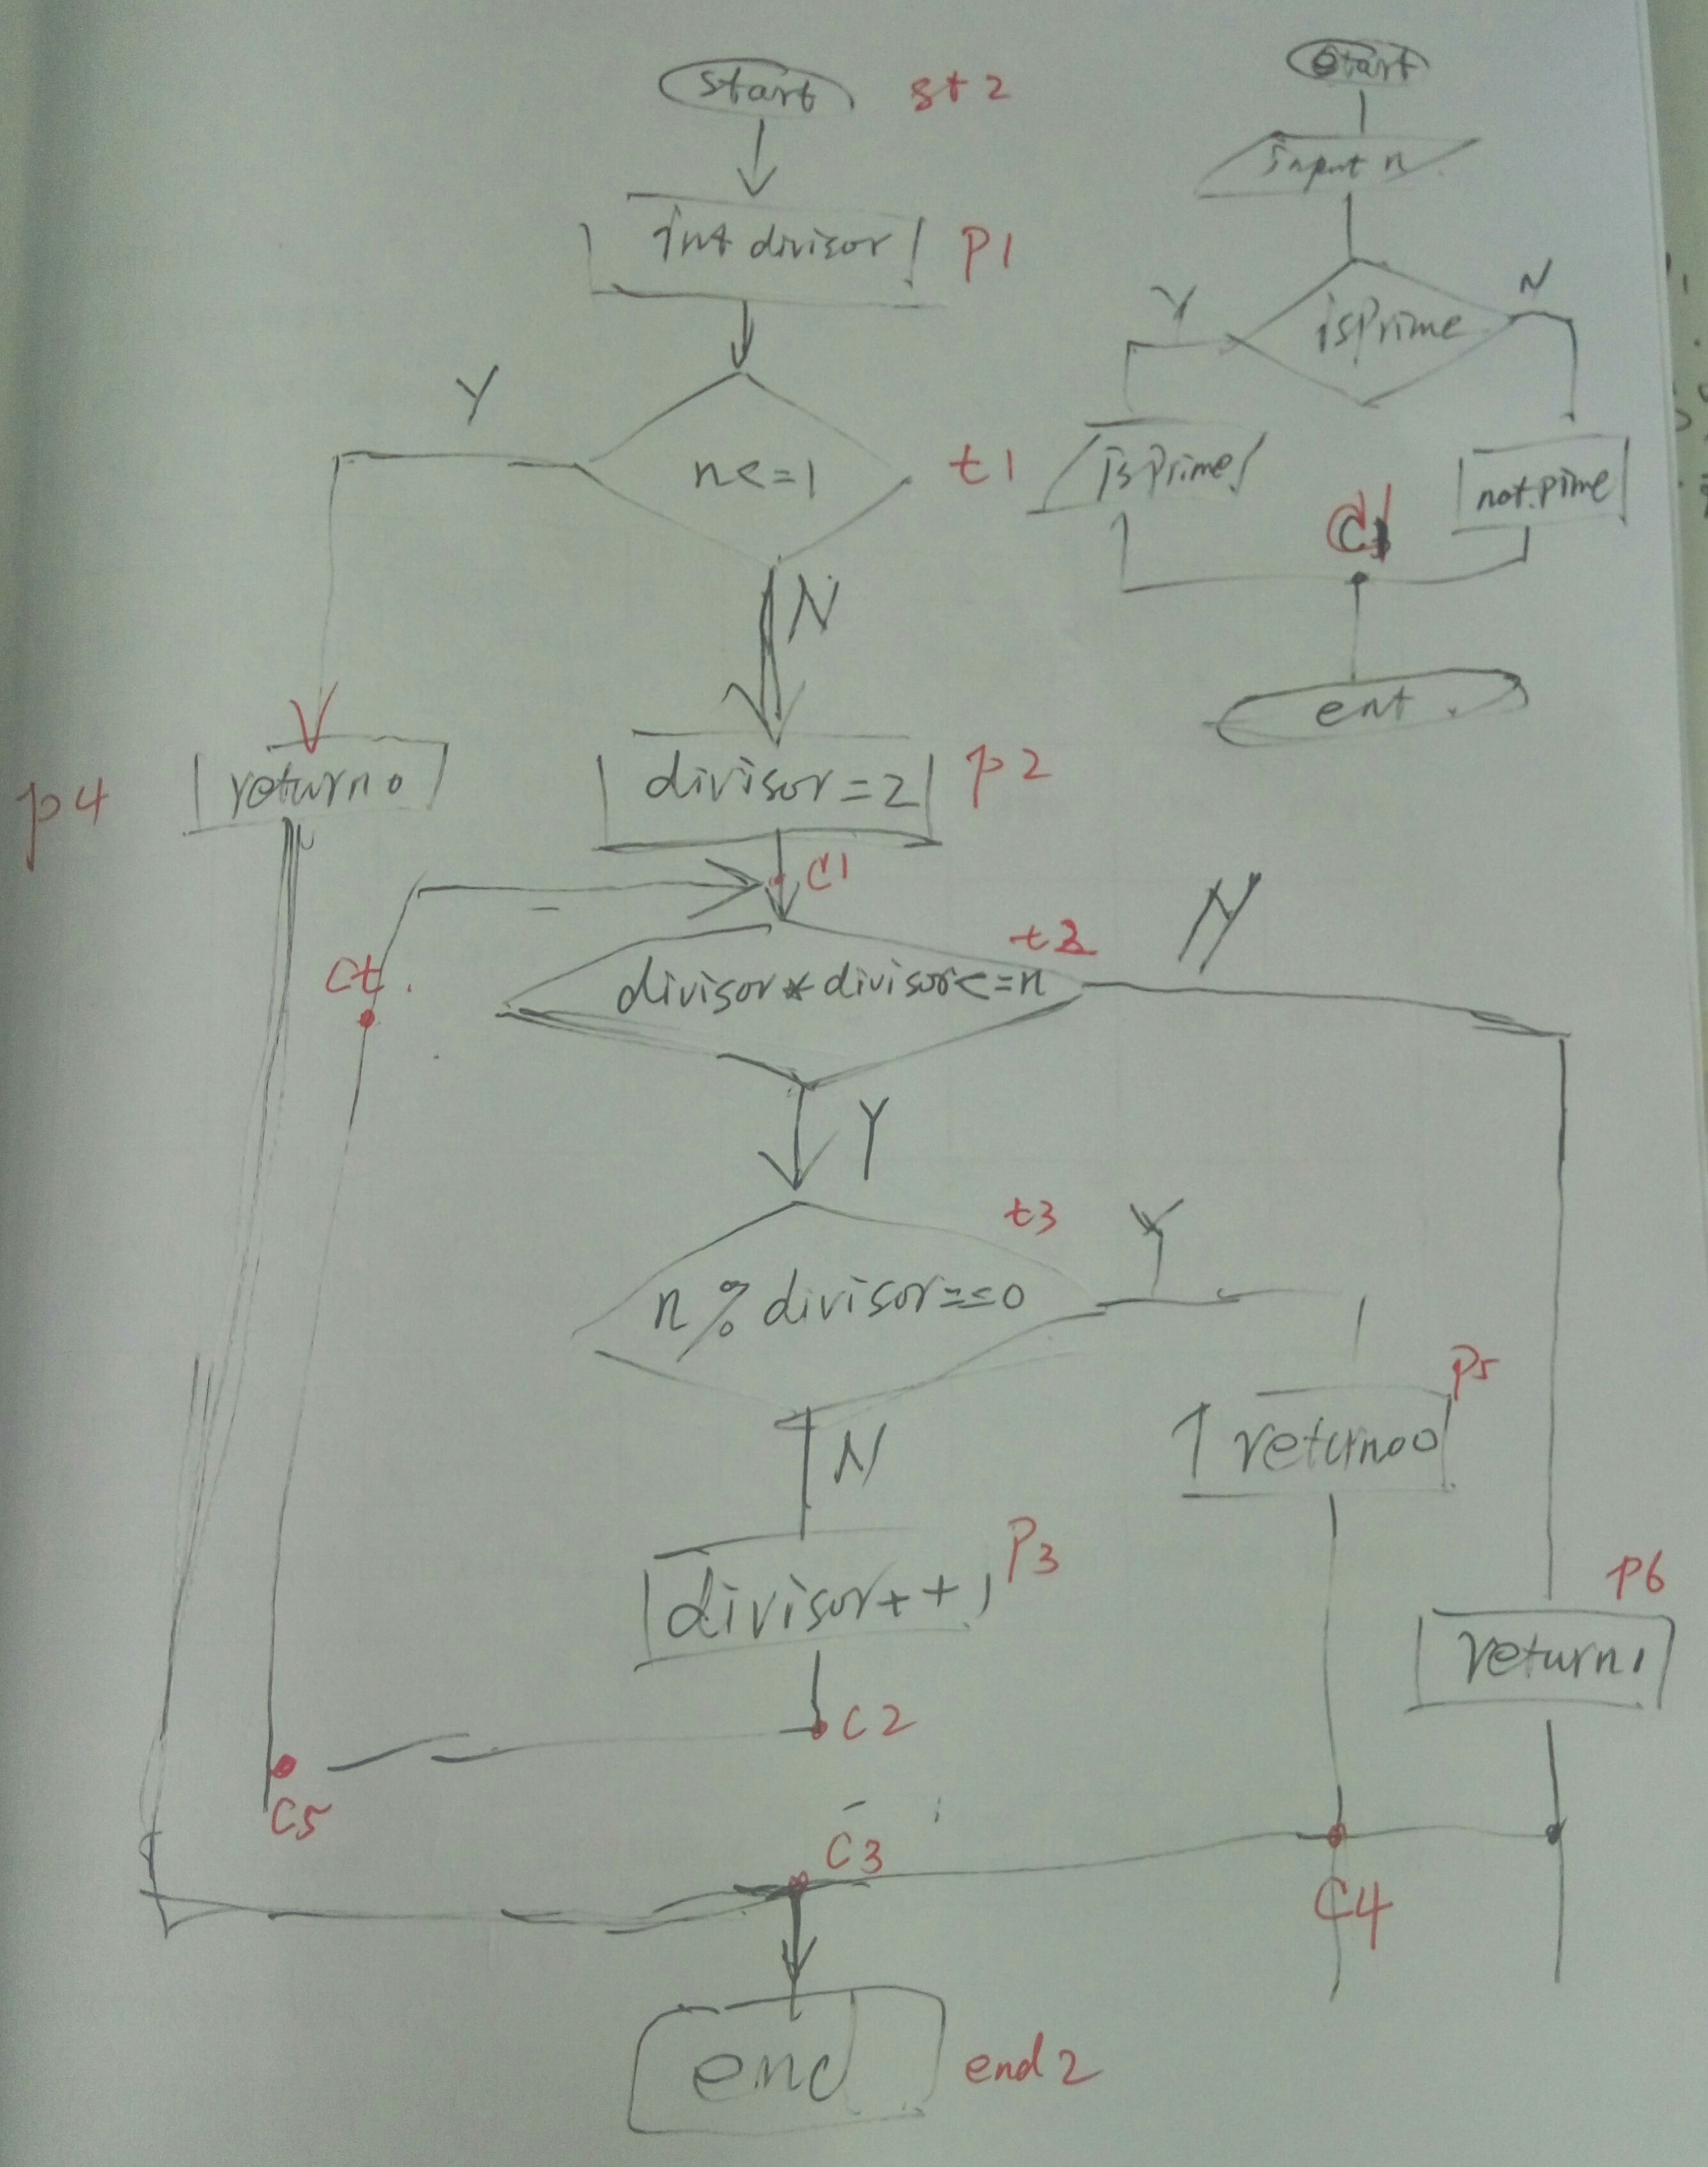
\includegraphics[width=0.35\textwidth]{02gcd}
      }{\caption{草图}\label{subfig:draft}}
      \ffigbox[\FBwidth]{
        \begin{tikzpicture}[scale=0.53,transform shape,]
          % 布置结点单元
          \node [term] (st) {开始};
          \node [proc, text width = 5em, join] (p1) {int divisor};       
          \node [test, join] (t1) {n <= 1};
          \node [proc, text width = 5em] (p2) {divisor = 2};
          \node [test, text width = 10em, join] (t2) {divisor * divisor <= n};
          \node [test, text width = 8em] (t3) {n \% divisor == 0};
          \node [proc, text width = 5em] (p3) {divisor++};
          \node [term, below = 1.6 of p3] (end) {结束};
          \node [proc, text width = 4em, left = 4.8 of t2] (p4) {return 0};
          \node [proc, text width = 4em, right = 3.5 of p3] (p5) {return 0};
          \node [proc, text width = 4em, right = 5.8 of t3] (p6) {return 1};

          % 布置用于连接的坐标结点,同时为其布置调试标记点。
          \node [coord] (c1) at ($(p2.south)!0.5!(t2.north)$)  {}; \cmark{1}
          \node [coord, below = 0.25 of p3] (c2)  {}; \cmark{2}
          \node [coord, above = 0.5 of end] (c3) {};  \cmark{3}
          \node [coord, left = 0.5 of t2] (ct) {};  \cmark{t}
          \node [coord] (c4) at (c3 -| p5)  {}; \cmark{4}
          \node [coord] (c5) at (c2 -| ct)  {}; \cmark{5}
        
          % 判断框连线,每次绘制时,先绘制一个带有一个固定
          % 位置标注的路径(path),然后再绘制箭头本身(arrow)。
          \path (t1.south) -- node [near start, right] {$N$} (p2.north);
          \draw [norm] (t1.south) -- (p2.north);
          \path (t1.west) -| node [near start, above] {$Y$} (p4.north);
          \draw [norm] (t1.west) -| (p4.north);
        
          \path (t2.south) -- node [near start, right] {$Y$} (t3.north);
          \draw [norm] (t2.south) -- (t3.north);
          \path (t2.east) -| node [near start, above] {$N$} (p6.north);
          \draw [norm] (t2.east) -| (p6.north);
        
          \path (t3.south) -- node [near start, right] {$N$} (p3.north);
          \draw [norm] (t3.south) -- (p3.north);
          \path (t3.east) -| node [near start, above] {$Y$} (p5.north);
          \draw [norm] (t3.east) -| (p5.north);

          % 其它连线
          \draw [norm](p3.south) |- (c5) |- (c1);
          \draw [norm](p4.south) |- (c3);
          \draw [norm](p4.south) |- (c3) -- (end);
          \draw [norm](p5.south) -- (c4);
          \draw [norm](p6.south) |- (c3);
          \draw [norm](p6.south) |- (c3) -- (end);
        \end{tikzpicture}
      }{\caption{TiKZ绘制图}\label{subfig:tikz}}
    \end{subfloatrow}
  }{\caption{用TiKZ绘制流程图}\label{fig:flowcharttikzdraw}}
\end{figure}

\subsection{UML图}
可以使用\enquote{pgf-umlcd}宏包实现UML图的绘制,在命令行
使用\enquote{texdoc pgf-umlcd}查看该宏包的使用说明书。

但由于TeXLive收集的pgf-umlcd宏包不能很好的处理中文类名,因此请使用模板
提供的pgf-umlcd宏包排版UML图。

\autoref{fig:uml}是使用\enquote{pgf-umlcd}宏包绘制的UML图。
\begin{figure}[!hpt]
  \centering
  \begin{tikzpicture}[font=\small]
    \tikzset{ coord/.style={coordinate} }    
    \begin{class}[fill=red!25, text width=7em]{动物类CAnimal}{0, 0}
      \attribute{-name[32]:char}
      \attribute{-age:int}
      \attribute{-weight:int}
      \operation{+show():void}
    \end{class}

    \begin{class}[fill=green!25, text width=5em]{马CHorse}{-5, -4.5}
      \inherit{动物类CAnimal}
      \attribute{-power:int}
      \operation{+show():void}
      \operation{+talk():void}
    \end{class}
      
    \begin{class}[fill=green!25, text width=5em]{鸟CBird}{0, -4.5}
      \inherit{动物类CAnimal}
      \attribute{-wingSpan:int}
      \operation{+show():void}
      \operation{+talk():void}
    \end{class}
      
    \begin{class}[fill=green!25, text width=5em]{牛CBull}{5, -4.5}
      \inherit{动物类CAnimal}
      \attribute{-power:int}
      \operation{+show():void}
      \operation{+talk():void}
    \end{class}

    \begin{class}[fill=blue!25, text width=6em]{飞马CPegasus}{-2.5, -8}
      \inherit{马CHorse}
      \inherit{鸟CBird}
      \operation{+show():void}
      \operation{+talk():void}
    \end{class}           
  \end{tikzpicture}  
  \caption{用\enquote{pgf-umlcd}宏包绘制UML图}\label{fig:uml}
\end{figure}

\subsection{代码排版}
在\enquote{nwafuprojrep.cls}模板中,可以引入了自己开发的boxie.sty宏包
进行代码排版。本文档\autoref{secboxiety}中有基本使用样例,详情请在\github{}查看
\href{https://github.com/registor/boxiesty}{boxie宏包}
的使用说明书。

\subsection{列表环境}
在\enquote{nwafuprojrep.cls}模板中,基于enumitem宏包分别对itemize、
enumerate和description三个环境的各个距离参数进行了修正,以使其排版结果
符合中文习惯的首先缩进格式。
\subsubsection{itemize环境}
\begin{itemize}
\item 床前明月光,床前明月光,床前明月光,床前明月光,床前明月光,床前明月光,床前明月光。
\item 疑是地上霜,疑是地上霜,疑是地上霜,疑是地上霜,疑是地上霜,疑是地上霜,疑是地上霜。
\item 举头望明月,举头望明月,举头望明月,举头望明月,举头望明月,举头望明月,举头望明月。
\item 低头思故乡,低头思故乡,低头思故乡,低头思故乡,低头思故乡,低头思故乡,低头思故乡。
\end{itemize}
\subsubsection{enumerate环境}
\begin{enumerate}
\item 床前明月光,床前明月光,床前明月光,床前明月光,床前明月光,床前明月光,床前明月光。
\item 疑是地上霜,疑是地上霜,疑是地上霜,疑是地上霜,疑是地上霜,疑是地上霜,疑是地上霜。
\item 举头望明月,举头望明月,举头望明月,举头望明月,举头望明月,举头望明月,举头望明月。
\item 低头思故乡,低头思故乡,低头思故乡,低头思故乡,低头思故乡,低头思故乡,低头思故乡。
\end{enumerate}
\subsubsection{description环境}
\begin{description}
\item[床前明月光],床前明月光,床前明月光,床前明月光,床前明月光,床前明月光,床前明月光。
\item[疑是地上霜],疑是地上霜,疑是地上霜,疑是地上霜,疑是地上霜,疑是地上霜,疑是地上霜。
\item[举头望明月],举头望明月,举头望明月,举头望明月,举头望明月,举头望明月,举头望明月。
\item[低头思故乡],低头思故乡,低头思故乡,低头思故乡,低头思故乡,低头思故乡,低头思故乡。
\end{description}

\subsection{\enquote{emph}强调字体}
在\enquote{nwafuprojrep.cls}模板中,重定义强调字体,将默认强调字体
是italic,中文用楷体代替操作更换为加粗操作,用加粗后的字体表示强调。
\subsection{文本框盒子}
文本框盒子继承于自己开发的boxie宏包,其使用细节请在\github{}查看
\href{https://github.com/registor/boxiesty}{boxie宏包}的使用说明书。
同时,在该宏包的基础上,为boxie宏包添加加了摘自于
\href{https://github.com/WisdomFusion/latex-templates/tree/master/progartcn}{progartcn
  论文模板}的\enquote{标题}、\enquote{注意}、\enquote{重要}、
\enquote{技巧}和\enquote{警告}文本框环境代码\footnote{本节示例摘自于
  该模板中的tutorial-sample.tex文件}。
\subsubsection{\enquote{标题}文本框}
标题文本框环境的使用格式为:

\verb|\begin{titledBox}{<title>} <content> \end{titledBox}|

\begin{titledBox}{HTTP/Console 内核}
  HTTP 内核继承自 \verb|Illuminate\Foundation\Http\Kernel| 类,该类定义了一个 \verb|bootstrappers| 数组,这个数组中的类在请求被执行前运行,这些 \verb|bootstrappers| 配置了错误处理、日志、检测应用环境以及其它在请求被处理前需要执行的任务。
\end{titledBox}
\subsubsection{\enquote{注意}文本框}
注意文本框环境的使用格式为:

\verb|\begin{noteBox} <content> \end{noteBox}|

\begin{noteBox}
  HTTP 内核继承自 \verb|Illuminate\Foundation\Http\Kernel| 类,该类定义了一个 \verb|bootstrappers| 数组,这个数组中的类在请求被执行前运行,这些 \verb|bootstrappers| 配置了错误处理、日志、检测应用环境以及其它在请求被处理前需要执行的任务。
\end{noteBox}

\subsubsection{\enquote{重要}文本框}
重要文本框环境的使用格式为:

\verb|\begin{importantBox} <content> \end{importantBox}|

\begin{importantBox}
  HTTP 内核继承自 \verb|Illuminate\Foundation\Http\Kernel| 类,该类定义了一个 \verb|bootstrappers| 数组,这个数组中的类在请求被执行前运行,这些 \verb|bootstrappers| 配置了错误处理、日志、检测应用环境以及其它在请求被处理前需要执行的任务。
\end{importantBox}
\subsubsection{\enquote{技巧}文本框}
技巧文本框环境的使用格式为:

\verb|\begin{tipBox} <content> \end{tipBox}|

\begin{tipBox}
  HTTP 内核继承自 \verb|Illuminate\Foundation\Http\Kernel| 类,该类定义了一个 \verb|bootstrappers| 数组,这个数组中的类在请求被执行前运行,这些 \verb|bootstrappers| 配置了错误处理、日志、检测应用环境以及其它在请求被处理前需要执行的任务。
\end{tipBox}
\subsubsection{\enquote{警告}文本框}
警告文本框环境的使用格式为:

\verb|\begin{warningBox} <content> \end{warningBox}|

\begin{warningBox}
  HTTP 内核继承自 \verb|Illuminate\Foundation\Http\Kernel| 类,该类定义了一个 \verb|bootstrappers| 数组,这个数组中的类在请求被执行前运行,这些 \verb|bootstrappers| 配置了错误处理、日志、检测应用环境以及其它在请求被处理前需要执行的任务。
\end{warningBox}

\subsection{交叉引用}
在技术文档中,图、表、公式等必须使用\emph{交叉引用},
在\enquote{nwafuprojrep.cls}模板中,交叉引用
用\verb|\autoref|命令实现引用,并对图、表、节、小节、公式、代码等引用
标记字/词进行了设置。如对一个标签为\enquote{fig:01}的图使用
\verb|\autoref{fig:01}|便可以得到\enquote{图 XX}的结果,用
\verb|\autoref{texcode01}|就可以得到\enquote{代码 XX}的结果。

\subsection{参考文献}
参考文献采用GB/T7714-2015标准的顺序编码制,使用biber+biblatex方式实现,
样式控制选择\enquote{biblatex-gb7714-2015}宏包的顺序编码制
(gb7714-2015)样式,如\autoref{texcode06}:

\begin{center}
  \begin{langCVOne}[tex][texcode06][\LaTeX{}]{引用参考文献}
    % 引用参考文献
    详见文献\cite{Peebles2001-100-100}\parencite{Babu2014--}
    另见文献\cite[49]{于潇2012-1518-1523}\parencite[106]{Babu2014--}
  \end{langCVOne}
\end{center}

能够生成如下引用结果:

% 引用参考文献
详见文献\cite{Peebles2001-100-100}\parencite{Babu2014--}
另见文献\cite[49]{于潇2012-1518-1523}\parencite[106]{Babu2014--}

\subsection{已载入的宏包}
在\enquote{nwafuprojrep.cls}模板中,已引入的宏包有:
\verb|etoolbox|、\verb|unicode-math|、\verb|geometry|、
\verb|graphicx|、\verb|fancyhdr|、\verb|titletoc|、
\verb|caption|、\verb|footmisc|、\verb|url|、
\verb|enumitem|、\verb|circledsteps|、\verb|filehook|,
无需再次引入这些宏包。

\subsection{重要文件}
\begin{importantBox}
  在使用在\enquote{nwafuprojrep.cls}模板前请确保:
  \verb|nwafuprojrep.cls|模板文件在当前工作文件夹中。
  
  如果需要代码盒子等各类盒子排版,则需要确保\verb|boxie.sty|、
  \verb|fvextra.sty|、\verb|lstlinebgrd.sty|
  这3个宏包文件在当前工作文件夹中,并且需要引入\verb|boxie|宏包,
  \verb|boxie|宏包会根据需要加载\verb|fvextra|和\verb|lstlinebgrd|
  宏包,这两个宏包无需手动加载。
  
  如果需要绘制UML图,则需要加载\verb|pgf-umlcd|宏包,此时需要确保\verb|pgf-umlcd.sty|
  宏包文件在当前工作文件夹中(TeXLive自带的宏包无法正确处理中文类名称,同时,
  修改了其association命令,以符合龚晓庆教材绘图习惯)。
  
  如果需要绘制流程图,则需要加载\verb|tikz-flowchart|宏包,此时需要确保\verb|tikz-flowchart.sty|
  宏包文件在当前工作文件夹中。
  
  如果需要为插图进行村注,则需要加载\verb|tikz-imglabels|宏包,此时需要确保\verb|tikz-imglabels.sty|
  宏包文件在当前工作文件夹中(TeXLive自带的宏包无法正确标注中的换行问题)。

  \verb|Makefile|文件是执行make命令需要的脚本文件,可以根据需要选择。

  \verb|.latexmkrc|文件是执行latexmk命令需要的脚本文件,可以根据需要选择。
\end{importantBox}

\subsection{排版编译}
\begin{importantBox}
  由于需要排版代码文件,建议使用minted宏包实现代码排版,因此请确保安装
  有Python及其Pygments模块,详情请使用\verb|texdoc minted|命令查看
  minted宏包的使用说明。

  同时,为支持minted编译,请使用\verb|-shell-escape|编译参数。  
\end{importantBox}

由于需要交叉引用和参考文献,建议按如下方式执行4次编译:

\subsubsection{使用minted宏包排版代码}
\begin{ubtdark}{4次编译}
  xelatex -shell-escape main.tex
  biber main
  xelatex -shell-escape main.tex
  xelatex -shell-escape main.tex
\end{ubtdark}

如果使用Makefile,则执行make命令即可:

\begin{ubtdark}{4次编译}
  make
\end{ubtdark}

如果使用\verb|.latexmkrc|,则执行latexmk命令即可:

\begin{ubtdark}{4次编译}
  latexmk
\end{ubtdark}

\subsubsection{使用listings宏包排版代码}
\begin{ubtdark}{4次编译}
  xelatex main.tex
  biber main
  xelatex main.tex
  xelatex main.tex
\end{ubtdark}

如果使用TeXstudio等IDE工具,请参阅相关资料对IDE进行必要的配置。

建议通过
\href{https://space.bilibili.com/1374419?from=search&seid=9480597470053264528}{
  王泽鹏老师的B站}资源,观看耿楠制作的教学视频学习必要的编译和配置过程。


\section{调试与测试}
该模板是第1次发布,仅进行了部分测试,还需要在使用中不断完善。如果发现
问题,请及时在gitee中提交issues,以便改进代码。

\section{实习日志}
实习日志用自定义的\enquote{logentry}环境编排,该环境第1个参数是日志标题
该参数为可选参数,第2个参数是日志日期,该参数为必选参数。
\begin{logentry}[会议讨论]{2020年6月17日}
  开会讨论,决定使用\LaTeX{}为实习报告排版提供支持,需要开发
  {nwafuprojrep.cls}模板。
\end{logentry}
\begin{logentry}[完成开发]{2020年6月28日}
  完成开发{nwafuprojrep.cls}模板v1.0.0开发,并进行了简单测试。在gitee平台
  开源发布\href{https://gitee.com/registor/nwafuprojrep}{nwafuprojrep v1.0.0模板}。  
\end{logentry}

\begin{logentry}[修正无Python的Pygments下代码排版问题]{2020年6月29日}
  在无Python的Pygments模块下,使用listings宏包实现代码排版,并在Windows平台下完成了
  测试,同时,发布nwafuprojrep模板v1.0.1版。  
\end{logentry}

\begin{logentry}[添加\enquote{logentry}日志环境]{2020年6月30日}
  为实习日志编写添加自定义\enquote{logentry}环境,该环境设计了2个参数,第1个参数是
  可选参数,用于排版日志标题;第2个参数是必选参数,用于排版日志日期。  
  
  同时,对\enquote{main.tex}说明文档进行了完善和修定,添加了UML图的绘制示例。
  
  将pgf-umlcd、floatrow、subcaptio、boxie、tikz-imglabels、
  tikz-flowchart宏包移出cls模板文件,以减少模板文档类的依赖,提高其灵活
  性。
  
  如果需要,需将这些宏包置于当前工作目录下,建议
  在settings/packages.tex文件中引用这引宏包,在settings/format.tex中进
  行\enquote{设置floatrow浮动体属性}、\enquote{代码交叉引用命
    令autoref的引用格式}等设置。当然,这些引用和设置也可以在导言区完
  成。

  同时,发布nwafuprojrep模板v1.0.2版。
\end{logentry}

\begin{logentry}[添加操作系统及字体判断功能]{2020年7月1日}
  借鉴zepinglee开发的\href{https://github.com/ustctug/ustcthesis}{中国科学技术大学学位论文\LaTeX{}模板}代码, 为\textbackslash{}nwafuset命令添加了操作系统和字体选择key-value选项,并实现了操作系统自动判断及字体自动选择功能。
\end{logentry}

\begin{logentry}[简化模板宏包依赖]{2020年7月2日}
  进一步简化了nwafuprojrep.cls中对其他宏包的依赖,仅添加必要和宏包。其他宏包由用户决定是否需要加载,建议按推荐的目录结构在settings/packages.tex中添加需要的宏包。
  
  添加报告(report)/论文(paper)选项,添加打印稿(print)/电子稿选项(epub)。
  
  添加摘要排版命令,实现摘要排版。
  
  修订README.md说明文件。
\end{logentry}

\section{实习总结}
通过本次实习,解决了广大学子在撰写实习报告时的排版问题,减轻了排版工作量,排版结果更标准、更专业......

\section{附录:核心代码清单}\label{secboxiety}
可以使用boxie宏包提供的langPyOne、langCVOne等环境或langPyfile和langCVfile
等命令实现嵌入式代码或来自文件代码的排版。Py系列环境和命令不带引用计数
和标签,CV系列环境和命令带有引用计数和标签。
\subsection{代码排版环境}
例如,使用langPyOne环境可以排版不带引用计数和标签的代码。
\begin{langPyOne}[C++]{基于范围的循环}
#include <iostream>
#include <vector>
using namespace std;
int main()
{
    // 累加 20 以内的素数
    int sum = 0;
    for(int e : {2, 3, 5, 7, 11, 13, 17, 19}) // 用 auto 类型更合理
    {
        sum += e;
    }
    cout << sum << endl;

    // 输出结果 77
    int arr[] = {1, 3, 5, 7, 9};
    // 声明数组 arr,初始化为 5 个奇数
    for(auto &ele : arr)
    {
        // 声明 ele,与数组 arr 关联在一起,用了 auto
        ele = ele * 2;
        // 修改数组每个元素的值
        cout << ele << " ";
        // 输出 ele,2 6 10 14 18
    }
    cout << endl;

    for(auto ele : arr)
    {
        cout << ele << " ";
    }
    // 没有改变:1 3 5 7 9
    cout << endl;

    return 0;
}  
\end{langPyOne}

再如,使用langCVOne环境可以排版带有引用计数和标签的代码,如\autoref{code:ex04-01}。
\begin{langCVOne}[C++][code:ex04-01][C++]{基于范围的循环}
#include <iostream>
#include <vector>
using namespace std;
int main()
{
    // 累加 20 以内的素数
    int sum = 0;
    for(int e : {2, 3, 5, 7, 11, 13, 17, 19}) // 用 auto 类型更合理
    {
        sum += e;
    }
    cout << sum << endl;

    // 输出结果 77
    int arr[] = {1, 3, 5, 7, 9};
    // 声明数组 arr,初始化为 5 个奇数
    for(auto &ele : arr)
    {
        // 声明 ele,与数组 arr 关联在一起,用了 auto
        ele = ele * 2;
        // 修改数组每个元素的值
        cout << ele << " ";
        // 输出 ele,2 6 10 14 18
    }
    cout << endl;

    for(auto ele : arr)
    {
        cout << ele << " ";
    }
    // 没有改变:1 3 5 7 9
    cout << endl;

    return 0;
}  
\end{langCVOne}

\subsection{代码排版命令}
代码排版命令用于根据代码文件进行排版,因此,可以在IDE中,例如
Code::Blocks中对代码进行排版,然后将排版后的文件直接用代码排版命令在
\LaTeX{}中进行排版。

例如,使用langPyfile命令可以载入代码文件,排版不带引用计数和标签的代码
(注意指定必要的路径)。

\langPyfile{基于范围的循环}{codes/ex04-01.cpp}

再如,使用langCVfile命令可以载入代码文件,排版带引用计数和标签的代码
(注意指定必要的路径),如\autoref{code:ex04-02}。

\langCVfile[C++][code:ex04-02][C++]{基于范围的循环}{codes/ex04-01.cpp}

注:使用minted宏包排版代码,可以使用c++/C++或cpp指定语言名称,若使
用listings宏包排版代码,则只能使用c++/C++指定语言名称

% 新起1页排版参考文献
\newpage
% 打印参考文献表
\printbibliography[heading=bibliography,title=参考文献]
\end{document}

%%% Local Variables:
%%% mode: latex
%%% TeX-master: t
%%% End:
